% \section{The reciprocal theorem and equaitons for a droplet force and Stresslet}
% \label{ap:reciprocal}




\section{Governing equations and fundamentals solutions}
\label{sec:governing_equation}

At the leading order in droplet volume fraction, the governing equations for $\textbf{u}^*$ and $p_f'$ are equivalent to that of an isolated droplet immersed in an infinite medium \citep{hinch1977averaged}. 
Hence, we consider the problem of an isolated test droplet immersed in an arbitrary flow where only the uniform relative motions induce inertia. 
The disturbances pressure and velocity fields ($\textbf{u}^*$ and $p_f'$), relative to the position of a test droplet are noted $\textbf{u}_{o}$, $\textbf{u}_{i}$, $p_{o}$ and $p_{i}$, for the velocity outside, and inside, the pressure outside and inside the volume of the test droplet, respectively. 
Recall that the center of mass velocity of the droplet is noted $\textbf{w}$. 
On~\ref{fig:disturbance} we display a schematic representation of the problem. 
\begin{figure}[h!]
    \centering
    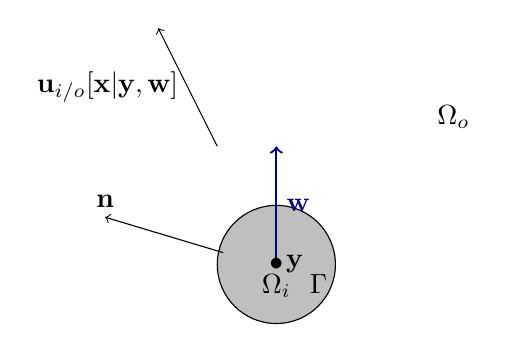
\begin{tikzpicture}[scale= 1.5]
        \filldraw[ gray!50!white](0,0)circle (0.5);
        \draw(0,0)circle (0.5)node[right,below]{   $\;\;\;\;\;\;\;\;\;\;\;\Gamma$};
        \draw[->,blue!50!black,thick](0,0)--++(0,1)node[midway,right]{$\textbf{w}$};
        \draw (0,0)node{$\bullet$}node[right]{$\textbf{y}$};
        \draw[->] (-0.45,0.1)--++(-1,0.3)node[above]{$\textbf{n}$};
        \draw[->](-0.5,1)--++(-0.5,1)node[midway,left]{$\textbf{u}_{i/o}[\textbf{x}|\textbf{y},\textbf{w}]$};
        % \draw[->] (3,1)node{$\bullet$}--++(0,1.5)node[right,midway]{$\textbf{u}_f[\textbf{x}]$};
        \draw (0,0)node[below]{$\Omega_i$};
        \draw (1.5,1.25)node{$\Omega_o$};
    \end{tikzpicture} 
    \caption{Representation of the problem parameters. $\textbf{u}_{o/i}[\textbf{x}|\textbf{y},\textbf{w}]$ is the disturbance velocity field evaluated at \textbf{x}, generated by a test droplet positioned at \textbf{y} with center of mass velocity \textbf{w}. \textbf{n} is the unit normal  pointing outward the droplet. 
    The domain of the exterior of the droplet is noted $\Omega_o$ and the one the interior $\Omega_i$.}
    \label{fig:disturbance}
\end{figure}

\subsection{Maxey, Riley \& Gatignol's equations}

Outside and inside the volume of the test droplet we can write the mass and momentum equations for the disturbances fields, that we noted $p_{o/i}$ and $\textbf{u}_{o/i}$, by conditionally averaging the Navier stokes equations \citep{koch1993hydrodynamic,fintzi2025}, or simply by considering the equations derived by~\cite{maxey1983equation} \& \citet{gatignol1983faxen}, both approach are equivalent\footnote{
    It must be noted that even in dilute systems, conditional averaging induces an additional stress in~\ref{eq:momentum_out} (see~\cite[Eq. (9)]{koch1993hydrodynamic}), which is not present in~\cite{maxey1983equation} \& \citet{gatignol1983faxen}'s equations. 
    This term corresponds to the velocity variance of the conditionally averaged velocity field (see \citet{koch1993hydrodynamic} or \citet[Chapter 4]{fintzi2025}), it is similar to the Reynolds Stress. 
    However, in this work, the turbulence considered is only the ``pseudo-turbulence'', hence it is $\propto \phi$ to some power. 
    Hence, in the conditionally averaged equations, this term turns out to be negligible \citep[Appendix A]{koch1993hydrodynamic}.
    In this context, conditionally averaged equations are equivalent to the equations for an isolated droplet. 
    The only difference is that conditionally averaged equations are explicitly related to ensemble averaged fields through their boundary conditions \citep{fintzi2025}. 
}. 
In dimensionless form they read, 
\begin{align}
    \div \textbf{u}_{o} &= 0
    \\
    \div\bm\sigma_{o}
    &= 
    Re [
    \pddt \textbf{u}_{o}
    + \textbf{u}_{o}\cdot \grad \textbf{u}_{o}
    + \textbf{u}_{o}\cdot \grad \textbf{w}_r
    + \textbf{w}_r \cdot \grad \textbf{u}_{o}]
    = Re \textbf{f}_{o},
    \label{eq:momentum_out}
\end{align}
for all $|\textbf{x}- \textbf{y}| = |\textbf{r}| = r > 1$, and, 
\begin{align}
    \div \textbf{u}_{i} &= 0,
    \\
    \div\bm\sigma_{i}
    &= 
    \frac{\zeta}{\lambda}Re [
    \pddt \textbf{u}_{i}
    + \textbf{u}_{i}\cdot \grad \textbf{u}_{i}
    + \textbf{u}_{i}\cdot \grad \textbf{w}_r 
    + \textbf{w}_r \cdot \grad \textbf{u}_{i}]
    = \frac{\zeta}{\lambda}Re \textbf{f}_{i},
    \label{eq:momentum_in}
\end{align}
for $r<1$. 
Here we introduced the notation $\textbf{w}_r = \textbf{u} - \textbf{w}$.  
We recall here that \textbf{u} is the undisturbed, or ensemble averaged velocity, governed by the ensemble averaged equations (from~\ref{eq:dt_phif} to~\eqref{eq:dt_uf2}).
Additionally, $\bm\sigma_{i/o} = -p_{i/o}\bm\delta + 2\textbf{e}_{i/o}$ with $\textbf{e}_{i/o} = \frac{1}{2}[\grad \textbf{u}_{i/o} + ^{\dagger}\grad \textbf{u}_{i/o}]$ is the dimensionless newtonian stresses in the interior and exterior of the test droplet. 
% We introduce the Reynolds number $Re = \frac{\rho_f a |\textbf{w}_r|}{\mu_f}$ based on the droplet radius $a$, the density ratio $\zeta = \rho_d / \rho_f$ and the viscosity ratio $\lambda = \mu_d / \mu_f$. 
Note that the distances have been made dimensionless using the radius $a$, and the velocities using the scale $U = |\textbf{w}_r|$, and the stresses using the scale $U\mu_f /a$. 
Because we neglected inertial effects generated due to linear and quadratic flows, as well as unsteady behaviors, the first and third term on the right-hand side of~\ref{eq:momentum_in,eq:momentum_out} will cancel in the calculation performed in~\ref{sec:compute_moments}. 


At the surface of the droplet ($r = 1$) the continuity of velocity and the non-deformability of the test droplet imposes, 
\begin{align}
    \textbf{u}_{i} - \textbf{u}_{o}= 0,
    && 
    (\textbf{u}_{i}+\textbf{w}_r) \cdot \textbf{n}
    =
    0.
    \label{eq:normal_vel}
\end{align} 
At the interface of the test droplet the absolutes tangential shear rates ($\textbf{e}_{i/o}+\textbf{E}$) are assumed continuous, however the disturbance shear rate $\textbf{e}_{i/o}$ is not. 
Recall that $\textbf{E} =\frac{1}{2} [\grad \textbf{u} + ^\dagger \grad \textbf{u}]$ is the ensemble averaged shear rate of the continuous phase.
Hence, the correct boundary condition for the disturbance shear rate is (at $r=1$),
\begin{equation}
    \mathbf{n}\cdot 2 [\textbf{e}_{o} - \lambda \textbf{e}_{i} + (1-\lambda)\textbf{E}
    % - \textbf{b}
    ]\cdot (\bm\delta - \textbf{nn})
    =
    \textbf{b}\cdot (\bm\delta - \textbf{nn}),
    % 0
    \label{eq:boundary_cdt_stress}
\end{equation}
with, 
\begin{equation}
    \textbf{b}
    =
    \frac{a \grad \gamma}{\mu_f |\textbf{w}_r|}. 
    % = Ma \grad\gamma /|\grad \gamma|. 
\end{equation}

Here we have considered Marangoni stresses in order to keep general when deriving the reciprocal relation (see~\ref{sec:reciprocal}), nevertheless $\textbf{b}$ will be taken to be zero in the final calculation of the moments \eqref{sec:compute_moments}. 
Note that for instance the ensemble averaged quantities $\textbf{u}$ and $\textbf{E}$ are kept general, hence their values depends on the position along the surface of the test droplet, thus $\textbf{w}_r[\textbf{r}]$ isn't a constant of space. 



Far from the test droplet it is assumed that the disturbance fields are statistically independent form the presence of the droplet, hence we have the following boundary condition far form the test drop,  
\begin{align}
    \lim_{r \to\infty }\textbf{u}_{o}[\textbf{r}|\textbf{y},\textbf{w}] = 0,
    && \lim_{r \to\infty }p_{o}[\textbf{r}|\textbf{y},\textbf{w}]= 0. 
    \label{eq:BC_r_infty_1}
\end{align}





\subsection{Stokes flow solution for a droplet embedded in a quadratic flow}
The Reciprocal theorem requires the use of a known solution.
We call that solution the \textit{test} solution, since its only purpose is to compute the \textit{real} solution of the equations introduced above. 
We note the \textit{test} velocity and stress fields $\hat{\textbf{u}}_{i/o}$ and $\hat{\bm\sigma}_{i/o} = - \hat{p}_{i/o}\bm\delta + \grad \hat{\textbf{u}}_{i/o} + ^\dagger\grad \hat{\textbf{u}}_{i/o}$, respectively. 
In general all the \textit{test} quantities are written with a hat. 

In this problem we neglect all inertial effects and consider an arbitrary quadratic flow. 
In this situation $\hat{p}_{o/i}$ and $\hat{\textbf{u}}_{o/i}$ satisfy,
\begin{align}
    \div \hat{\textbf{u}}_{o} = 0 
    &&\div\hat{\bm\sigma}_{o}  = 0 
    \label{eq:momentum_out_s}\\
    \div \hat{\textbf{u}}_{i} = 0 
    && \div\hat{\bm\sigma}_{i}  = 0 
    \label{eq:momentum_in_s}
\end{align}
with the boundary conditions, 
\begin{align}
    \lim_{r \to\infty }\hat{\textbf{u}}_{o}[\textbf{r}|\textbf{y},\textbf{w}] = 0,
    && \lim_{r \to\infty }\hat{p}_{o}[\textbf{r}|\textbf{y},\textbf{w}]= 0. 
    \label{eq:BC_r_infty_2}
\end{align}
and (at $r=1$),
\begin{align}
    \label{eq:normal_vel2_s}
    \hat{\textbf{u}}_{i} &= \hat{\textbf{u}}_{o}\\
    \hat{\textbf{u}}_{i} \cdot \textbf{n} &= - \hat{\textbf{w}}_r \cdot \textbf{n}
    \label{eq:normal_vel_s}
    \\
    \label{eq:normal_stres_s}
    \mathbf{n}\cdot 2[\hat{\textbf{e}}_{o} - \lambda \hat{\textbf{e}}_{i} + (1-\lambda) \hat{\textbf{E}}
    % - \hat{\textbf{b}}
    ]\cdot (\bm\delta - \textbf{nn})
    &=
    \hat{\textbf{b}}\cdot (\bm\delta - \textbf{nn})
    % 0
\end{align}
where we introduced $\hat{\textbf{w}}_r = \hat{\textbf{u}} - \textbf{w}$ as the undisturbed relative velocity field of the test problem, similarly $\hat{\textbf{E}}$ is the undisturbed stress of the test problem. 
Note that for the test problem it is important that $\hat{\textbf{b}}\neq 0$, this will be useful to write the reciprocal relation in~\ref{sec:reciprocal}.


For our purposes we only need $\hat{\textbf{b}}$ and $\hat{\textbf{u}}$ to be quadratic fields.
Hence, we consider the relations, 
\begin{align}
    \hat{\textbf{w}}_r(\textbf{y} + \textbf{r}) 
    &=  \hat{\textbf{w}}_r|_{\textbf{r}=0}
    +  \textbf{r} \cdot  \grad\hat{\textbf{u}}|_{\textbf{r}=0}
    +  \frac{1}{2}\textbf{rr} :  \grad\grad\hat{\textbf{u}}|_{\textbf{r}=0}
    \label{eq:w_r_expand}\\
     \hat{\textbf{E}}(\textbf{y} + \textbf{r}) 
    &=   \hat{\textbf{E}}|_{\textbf{r}=0}
    + \textbf{r} \cdot  \grad \hat{\textbf{E}}|_{\textbf{r}=0}
    %+ \frac{1}{2}\textbf{rr} :  \grad\grad \hat{\textbf{E}}|_{\textbf{r}=0}
    \\
     \hat{\textbf{b}}(\textbf{y} + \textbf{r}) 
    &=   \hat{\textbf{b}}|_{\textbf{r}=0}
    + \textbf{r} \cdot  \grad \hat{\textbf{b}}|_{\textbf{r}=0}
    + \frac{1}{2}\textbf{rr} :  \grad\grad \hat{\textbf{b}}|_{\textbf{r}=0}
\end{align}
% \tb{note that we don't consider the symmetry between gradient hence $\grad\grad\hat{\textbf{u}}\approx $ arbitrary tensor; this is already what is considered }

According to the linearity of the Stokes equations~\ref{eq:momentum_out_s,eq:momentum_in_s}, and of the boundary conditions~\ref{eq:normal_vel2_s,eq:normal_vel_s,eq:normal_stres_s} we deduce that $\hat{\textbf{u}}_{i/o}$ and $\hat{p}_{i/o}$  must be linear combination of spherical harmonics proportional to $\hat{\textbf{w}}_r|_{\textbf{r}=0}$, $\hat{\textbf{b}}|_{\textbf{r}=0}$, and their derivatives \citep{brenner1963resistance}.
Hence, we can write the general solution of $\textbf{u}_{i/o}$ and $p_{i/o}$ as,
\begin{align}
    \begin{pmatrix}
        \hat{\textbf{u}}_{o}\\
        \hat{p}_{o}\\
        \hat{\textbf{u}}_{i}\\
        \hat{p}_{i}
    \end{pmatrix}
    =
    \begin{pmatrix}
        \textbf{U}_{o}^{(1)} + \textbf{U}_{o}^{(2)}\cdot \grad + \textbf{U}_{o}^{(3)} :\grad\grad &
        \textbf{U}_{o}^\text{(1-b)} + \textbf{U}_{o}^\text{(2-b)}\cdot \grad + \textbf{U}_{o}^\text{(3-b)} :\grad\grad \\
        \textbf{P}_{o}^{(1)} + \textbf{P}_{o}^{(2)}\cdot \grad + \textbf{P}_{o}^{(3)} :\grad\grad &
        \textbf{P}_{o}^\text{(1-b)} + \textbf{P}_{o}^\text{(2-b)}\cdot \grad + \textbf{P}_{o}^\text{(3-b)} :\grad\grad \\
        \textbf{U}_{i}^{(1)} + \textbf{U}_{i}^{(2)}\cdot \grad + \textbf{U}_{i}^{(3)} :\grad\grad &
        \textbf{U}_{i}^\text{(1-b)} + \textbf{U}_{i}^\text{(2-b)}\cdot \grad + \textbf{U}_{i}^\text{(3-b)} :\grad\grad \\
        \textbf{P}_{i}^{(1)} + \textbf{P}_{i}^{(2)}\cdot \grad + \textbf{P}_{i}^{(3)} :\grad\grad &
        \textbf{P}_{i}^\text{(1-b)} + \textbf{P}_{i}^\text{(2-b)}\cdot \grad + \textbf{P}_{i}^\text{(3-b)} :\grad\grad \\
    \end{pmatrix}
    \cdot 
    \begin{pmatrix}
        \hat{\textbf{w}}_r\\
        \hat{\textbf{b}}
    \end{pmatrix}
    \label{eq:big_solution}
\end{align}
The tensor $\textbf{U}_{i/o}^{(n)}$ and $\textbf{P}_{i/o}^{(n)}$ are $n+1$ and $n$ order tensors given in \citet[Appendix F]{fintzi2025averaged}, that depend only on the relative coordinate $\textbf{r} = \textbf{x}-\textbf{y}$ and the viscosity ratio $\lambda$.
We also define the $n+2$ order tensors, 
\begin{equation}
    \textbf{S}_{i/o}^{(n)} = 
    - \bm\delta\textbf{P}_{i/o}^{(n)}
    + \grad \textbf{U}_{i/o}^{(n)}
    + ^\dagger\grad \textbf{U}_{i/o}^{(n)},
    \label{eq:big_S}
\end{equation}\footnote{The $^\dagger$ used in~\ref{eq:big_S} represents the transpose operator which acts on the two closet index.
For example, the transpose of the triadic $\textbf{abc}$, may be written:  $^\dagger\textbf{abc} = \textbf{bac}$ or $\textbf{abc}^\dagger = \textbf{acb}$. }
where $n =1,2,3$ or $1\text{-}b,2\text{-}b,3\text{-}b$. 
\ref{eq:big_S} provides the stresses fields of the test problem upon contraction with $\hat{\textbf{w}}_r$, and $\hat{\textbf{b}}$, and the higher derivatives. 

\subsection{Singularity solutions}

Following \citet{stone2001inertial} we also consider the test problem of a point source located at the origin.
The reason why this solution is necessary is because, in the previous test problem $\div \hat{\textbf{u}}= 0$, hence the previous solution was unable to provide a formula for the trace of the first moment using the reciprocal theorem.
Because we also aim to compute the traces of the second moment of force one also need solution of point forces and potential dipole.  
These two classes of solutions, i.e., point force and point source, obey   the non-homogeneous Stokes equations, 
\begin{align}
    \grad^2 \hat{\textbf{u}}_o = \grad \hat{p}_o + (\textbf{Q}^{(n)}\otimes \grad^{(n)})\grad \delta(\textbf{r}),
    &&
    \grad^2 \hat{\textbf{u}}_o = \grad \hat{p}_o + (\textbf{B}^{(n+1)}\otimes \grad^{(n)}) \delta(\textbf{r}),
\end{align}
respectively. 
Where $\textbf{Q}^{(n)}$ and $\textbf{B}^{(n+1)}$ are two arbitrary $n^{th}$ and $(n+1)^{th}$ order tensors, respectively. 
Similarly the $\grad^{(n)}$ denote $n^{th}$ order outter product of gradients vectors.
The operator $\otimes$ represents the contraction product on the $n^{th}$ common indices. 
Both equations are completed by the continuity equation $\div \textbf{u}_{o}$. 
The solution of the point source, and point forces equations read, 
\begin{align}
    \hat{\textbf{u}}_o = -\frac{1}{4\pi}\grad^{(n+1)}(1/r)\otimes \textbf{Q}^{(n)}
    \label{eq:pts_source_n}
    &&
    \hat{\textbf{u}}_o = \frac{1}{8\pi}\grad^{(n)}[\grad^{(2)} - \bm\delta \grad^2]r
    \otimes \textbf{B}^{(n+1)}
\end{align}
The Stresses tensors read, 
\begin{align}
    \hat{\bm\sigma}_o = -\frac{1}{2\pi}\grad^{(n+2)}(1/r)\otimes \textbf{Q}^{(n)}, 
    &&
    \hat{\bm\sigma}_o = \frac{1}{8\pi}\grad^{(n)}[
        2\grad^{(3)}
        -(\grad \bm\delta + ^\dagger\grad\bm\delta+\bm\delta \grad)\grad^2
    ]r\otimes \textbf{B}^{(n+1)},
\end{align}
for the point source and point forces solutions, respectively. 
More details on how to obtain those solutions are given in~\citet[Chapter 6]{pozrikidis2011introduction} or in~\ref{ap:singularity_sol}. 

As an example, the solutions of a point source (i.e.,~\ref{eq:pts_source_n} with $n=0$) used in the calculation of the first moment of force reads, 
\begin{align}
    \hat{\textbf{u}}_{o} = \frac{Q^{(0)}}{4\pi} \textbf{n}r^{-2}
    && \hat{\bm\sigma}_{o} = \mu_f \frac{Q^{(0)}}{2\pi}\left(
        \bm\delta
        - 3 \textbf{nn}
    \right)r^{-3}
    \label{eq:point_source}
\end{align}
Note that this expression is valid throughout the domain excluding the point $\textbf{r} =  \textbf{x} -  \textbf{y} = 0$, hence we may use either the subscript $o$ or $i$. 
Point source dipole, and point force will also be used to derive relations for the traces of the second moment of force. 


In summary, as the values of $\hat{\textbf{w}}_r$, $\hat{\textbf{b}}$, $\textbf{B}^{(n)}$, and $\textbf{Q}^{(n)}$, are entirely arbitrary, the solutions given by~\ref{eq:big_solution,eq:pts_source_n,eq:point_source} can be used as a tool to derive formula for the drag forces, first moment, and second moment of hydrodynamic forces, using the reciprocal theorem derived in~\ref{sec:reciprocal}.  

\section{Reciprocal theorem for droplets}
\label{sec:reciprocal}

A similar derivation of what is presented here may be found in \citet{lovalenti1993force,raja2010inertial}, however we provide some clarifications by exposing a detailed and  (we hope) simpler demonstration, which remains more general because it provides a formula for the second moments of force.  

The derivation of the general formula goes into three steps: (1) we write a reciprocal relation in the exterior of the test droplet, (2) then on the interior of the test  droplet, and (3) then using the boundary condition at the interface of the droplet we write the final reciprocal relation that is referred to as reciprocal theorem. 

\subsection{First step:}
We first take the dot product of~\ref{eq:momentum_out} with $\hat{\textbf{u}}_{o}$, and the dot product of~\ref{eq:momentum_out_s} with $\textbf{u}_{o}$, subtracting both expression gives, 
\begin{equation}
    \div (\bm\sigma_{o}\cdot \hat{\textbf{u}}_o)
    % - \bm\sigma_o :\grad \hat{\textbf{u}}_o
    % \hat{\textbf{u}}_{o} \cdot (\div \bm\sigma_{o})
    =
    \div (\hat{\bm\sigma}_{o}\cdot \textbf{u}_o)
    % - \hat{\bm\sigma}_o :\grad \textbf{u}_o
    + Re (\hat{\textbf{u}}_{o}\cdot \textbf{f}_{o}). 
    \label{eq:first_step_out}
\end{equation}
To derive this relation we used the fact that $\bm\sigma_o :\grad \hat{\textbf{u}}_o = 2\textbf{e}_o :\grad \hat{\textbf{u}}_o = 2{\textbf e}_o : \hat{\textbf e}_o$, and  $\hat{\bm\sigma}_o :\grad {\textbf{u}}_o = 2\hat{\textbf{e}}_o : \textbf{e}_o$, leading to $\bm\sigma_o :\grad \hat{\textbf{u}}_o = \hat{\bm\sigma}_o :\grad {\textbf{u}}_o$. 
This simplification is the reason why the complete knowledge of the velocity field in the exterior of the droplet becomes unnecessary when $\textbf{f}_o = 0$.
Consequently, the  efficiency of the reciprocal theorem is rooted in the commutativity of the operation $\textbf e_o:\hat{\textbf e}_o$. 
Integrating this expression on the whole domain $\Omega_{o}$, and injecting the relations $\textbf{u}_o = \textbf{u}_o+\textbf{w}_r-\textbf{w}_r$ and $\hat{\textbf{u}}_o = \hat{\textbf{u}}_o+\hat{\textbf{w}}_r-\hat{\textbf{w}}_r$ gives, 
\begin{equation}
    \intS[p]{\hat{\textbf{w}}_{r} \cdot  \bm\sigma_{o}\cdot \textbf{n}}
    - 2\intS[p]{(\hat{\textbf{u}}_{o} + \hat{\textbf{w}}_r) \cdot  \textbf e_{o}\cdot \textbf{n}}
    =
    \intS[p]{\textbf{w}_{r}\cdot \hat{\bm\sigma}_{o}\cdot \textbf{n}}
    - 2\intS[p]{(\textbf{u}_{o} + \textbf{w}_r)\cdot \hat{\textbf e}_{o}\cdot \textbf{n}}
    + 
    Re\intO[o]{\hat{\textbf{u}}_{o}\cdot \textbf{f}_{o}}.
    \label{eq:int_first_step}
\end{equation}
Where we used the relation, $(\hat{\textbf{u}}_{o} + \hat{\textbf{w}}_r) \cdot  \bm\sigma_{o}\cdot \textbf{n} = 2 (\hat{\textbf{u}}_{o} + \hat{\textbf{w}}_r) \cdot  \textbf e_{o}\cdot \textbf{n}$, allowed  because $(\hat{\textbf{u}}_{o} + \hat{\textbf{w}}_r) = (\bm\delta - \textbf{nn})\cdot (\hat{\textbf{u}}_{o} + \hat{\textbf{w}}_r)$ on the surface of the test droplet, see~\ref{eq:normal_vel_s}. 
Similar considerations lead to $({\textbf{u}}_{o} + {\textbf{w}_r}) \cdot  \hat{\bm\sigma}_{o}\cdot \textbf{n} =2  ({\textbf{u}}_{o} + {\textbf{w}_r}) \cdot  \hat{\textbf e}_{o}\cdot \textbf{n}$. 
The surface integrals appear only on the surface of the test droplets because far from the test droplet ($r\to\infty$), $\hat{\textbf{u}}_o$, $\hat{\bm\sigma}_o$, $\textbf{u}_o$ and $\bm\sigma_o$ cancel out (see~\ref{eq:BC_r_infty_1} and~\ref{eq:BC_r_infty_2}). 

\ref{eq:int_first_step} is the correct reciprocal relation if one considers solid particles.
Indeed, in that case $\textbf{u}_{o}+\textbf{w}_r = 0$, and $\hat{\textbf{u}}_{o}+\hat{\textbf{w}}_r = 0$ at $r=1$, because of the no-slip boundary condition at the particle interface, hence leading directly to a formula for the force traction on the surface of the solid particle (first term on the left-hand side of~\ref{eq:int_first_step}).
Of course, one still needs to provide an approximation for $\textbf{f}_o$ if inertia is considered. 
For fluid particles a few more steps are necessary. 

\subsection{Second step:}

We now take the dot product of~\ref{eq:momentum_in} with $(\hat{\textbf{u}}_i + \hat{\textbf{w}}_r)$ and of~\ref{eq:momentum_in_s} with $(\textbf{u}_i+ \textbf{w}_r)$, subtracting both expression leads to, 
\begin{equation}
    \div [\bm\sigma_{i}\cdot (\hat{\textbf{u}}_i+\hat{\textbf{w}}_r)]
    - 2\textbf{e}_i : \hat{\textbf{E}}
    % \hat{\textbf{u}}_{i} \cdot (\div \bm\sigma_{i})
    =
    \div [\hat{\bm\sigma}_{i}\cdot (\textbf{u}_i+\textbf{w}_r)]
    - 2\hat{\textbf{e}}_i :\textbf{E}
    + \frac{\zeta}{\lambda} Re (\hat{\textbf{u}}_i+\hat{\textbf{w}}_r)\cdot \textbf{f}_{i}. 
    \label{eq:second_step_out}
\end{equation}
where we used the relation, $- \bm\sigma_i :\grad (\hat{\textbf{u}}_i+\hat{\textbf{w}}_r)+ \hat{\bm\sigma}_i :\grad ({\textbf{u}}_i+{\textbf{w}}_r) =
- 2\textbf{e}_i :\hat{\textbf{E}} + 2\hat{\textbf{e}}_i :\textbf{E}$. 
% We recall that $\hat{\bm\tau}_f$ and $\bm\tau_f$ correspond to the ensemble averaged stress fields of the test problem and true problem, respectively. 
Integrating this relation over the domain $\Omega_i$, and using the divergence theorem, as well as similar simplifications used in~\ref{eq:int_first_step}, gives, 
\begin{equation}
    \intS[p]{ (\hat{\textbf{u}}_i+\hat{\textbf{w}}_r)\cdot \textbf{e}_{i}\cdot\textbf{n}}
    - \intO[i]{\textbf{e}_i : \hat{\textbf{E}}}
    =
    \intS[p]{ (\textbf{u}_i+\textbf{w}_r)\cdot\hat{\textbf{e}}_{i}\cdot \textbf{n}}
    - \intO[i]{\hat{\textbf{e}}_i :\textbf{E}}
    + \frac{\zeta}{2\lambda} Re \intO{(\hat{\textbf{u}}_i+\hat{\textbf{w}}_r)\cdot \textbf{f}_{i}} 
    \label{eq:second_step_int}
\end{equation}
Because $(\hat{\textbf{u}}_i+\hat{\textbf{w}}_r)\cdot (\bm\delta-\textbf{nn}) = (\hat{\textbf{u}}_i+\hat{\textbf{w}}_r)$, multiplying~\ref{eq:boundary_cdt_stress} by $(\hat{\textbf{u}}_i+\hat{\textbf{w}}_r)$ gives the appropriate boundary condition for the first integral on the left-hand side of~\ref{eq:second_step_int}, namely,
\begin{equation}
    \mathbf{n}\cdot 2[
        \textbf{e}_{o} - \lambda \textbf{e}_i 
        + (1 -\lambda) \textbf{E}
        % - \textbf{b}
        ]\cdot (\hat{\textbf{u}}_{i/o}+\hat{\textbf{w}}_r)
        =
        \textbf{b}\cdot (\hat{\textbf{u}}_{i/o}+\hat{\textbf{w}}_r)
    \label{eq:boundary_with_the_velocity}
\end{equation}
with a similar relation for the test problem boundary condition and $({\textbf{u}}_{i/o}+{\textbf{w}}_r)$ in the first integral on the right-hand side of~\ref{eq:second_step_int}. 

Adding~\ref{eq:int_first_step} and~\ref{eq:second_step_int} times $2\lambda$, while using the boundary condition given by~\ref{eq:boundary_with_the_velocity} leads to the expression,
\begin{multline}
    \intS[p]{\hat{\textbf{w}}_{r} \cdot  \bm\sigma_{o}\cdot \textbf{n}}
    -\lambda \intO[i]{2\textbf{e}_i : \hat{\textbf{E}}}
    - (1-\lambda) \intS[p]{2(\textbf{u}_{i} + \textbf{w}_r)\cdot \hat{\textbf{E}}\cdot \textbf{n}}
    + \intS[p]{(\textbf{u}_{i} + \textbf{w}_r)\cdot \hat{\textbf{b}}}
    \\
    =
    \intS[p]{\textbf{w}_{r}\cdot \hat{\bm\sigma}_{o}\cdot \textbf{n}}
    - \lambda \intO[i]{2\hat{\textbf{e}}_i :\textbf{E}}
    - (1-\lambda) \intS[p]{2(\hat{\textbf{u}}_{i} + \hat{\textbf{w}}_r) \cdot  \textbf{E} \cdot \textbf{n}}\\ 
    + \intS[p]{(\hat{\textbf{u}}_{i} + \hat{\textbf{w}}_r) \cdot  \textbf{b}}
    + \zeta Re \intO{(\hat{\textbf{u}}_i+\hat{\textbf{w}}_r)\cdot \textbf{f}_{i}} 
    + Re\intO[o]{\hat{\textbf{u}}_{o}\cdot \textbf{f}_{o}}.
    \label{eq:int_third_step}
\end{multline}

\subsection{Final step:}

To obtain the ``final form'' of the reciprocal theorem we proceed by noting that the second and third terms on the left-hand side  of~\ref{eq:int_third_step} may be combined upon using the divergence theorem on the third term, and using the relation, 
\begin{equation}
    - \lambda \textbf{e}_i : \hat{\textbf{E}}
    - (1-\lambda)\div [\hat{\textbf{E}} \cdot (\textbf{u}_i + \textbf{w}_r)]
    =
    % - \lambda \textbf{e}_i : \hat{\textbf{E}}
    % - (1-\lambda) \hat{\textbf{E}}:(\textbf{e}_i + \textbf{E})
    - \textbf{e}_i : \hat{\textbf{E}}
    - (1-\lambda) \hat{\textbf{E}}:\textbf{E}
    - (1-\lambda)\div \hat{\textbf{E}} \cdot (\textbf{u}_i + \textbf{w}_r).
    \label{eq:tricks_two}
\end{equation}
One can also derive the same manipulation on the second and third term on the right-hand side of~\ref{eq:int_third_step}, namely,
\begin{equation}
    - \lambda \hat{\textbf{e}}_i : {\textbf{E}}
    - (1-\lambda)\div [{\textbf{E}} \cdot (\hat{\textbf{u}}_i + \hat{\textbf{w}}_r)]
    =
    % - \lambda \textbf{e}_i : \hat{\textbf{E}}
    % - (1-\lambda) \hat{\textbf{E}}:(\textbf{e}_i + \textbf{E})
    - \hat{\textbf{e}_i} : {\textbf{E}}
    - (1-\lambda) \hat{\textbf{E}}:\textbf{E}
    - (1-\lambda)\div {\textbf{E}} \cdot (\hat{\textbf{u}}_i + \hat{\textbf{w}}_r)
    \label{eq:tricks_one}
\end{equation}
Because the product $\hat{\textbf{E}} : {\textbf{E}}$ is commutative, the second term on the right-hand side of~\ref{eq:tricks_one} and~\ref{eq:tricks_two} cancel each other in the final expression.  
Injecting both~\ref{eq:tricks_one} and~\ref{eq:tricks_two} in~\ref{eq:int_third_step} leads to the final form of the reciprocal theorem for droplets, 
\begin{multline}
    \intS[p]{\hat{\textbf{w}}_{r} \cdot  \bm\sigma_{o}\cdot \textbf{n}}
    - \intO[i]{2\textbf{e}_i : \grad\hat{\textbf{u}}}
    - (1-\lambda) \intO[i]{(\textbf{u}_{i} + \textbf{w}_r)\cdot \grad^2 \hat{\textbf{u}}}
    + \intS[p]{(\textbf{u}_{i} + \textbf{w}_r)\cdot \hat{\textbf{b}}}
    \\
    =
    \intS[p]{\textbf{w}_{r}\cdot \hat{\bm\sigma}_{o}\cdot \textbf{n}}
    - \intO[i]{2\hat{\textbf{e}}_i :\grad\textbf{u}}
    - (1-\lambda) \intO[i]{(\hat{\textbf{u}}_{i} + \hat{\textbf{w}}_r) \cdot \grad^2 \textbf{u} }\\ 
    + \intS[p]{(\hat{\textbf{u}}_{i} + \hat{\textbf{w}}_r) \cdot  \textbf{b}}
    + \zeta Re \intO{(\hat{\textbf{u}}_i+\hat{\textbf{w}}_r)\cdot \textbf{f}_{i}} 
    + Re\intO[o]{\hat{\textbf{u}}_{o}\cdot \textbf{f}_{o}}.
    \label{eq:int_final_step}
\end{multline}
Note that we used the relations, $2{\textbf{e}_i} : \hat{\textbf{E}} = 2{\textbf{e}_i} : {\grad\textbf{u}}$ and $\div\textbf{E} = \frac{1}{2}\grad^2 \textbf{u}$ because the background flow is divergence free~\eqref{eq:div_u}. 
Upon making the good choice for $\hat{\textbf{w}}_r$ and $\hat{\textbf{b}}$ (i.e. whether it is constant, linear, or quadratic, see~\ref{eq:w_r_expand}), one recovers on the left-hand side of~\ref{eq:int_final_step} the expression of the force, first, and second moments applied on the droplet in a yet arbitrary flow described by $\textbf{u}$ and $\textbf{b}$. 

On the right-hand side of~\ref{eq:int_final_step} all the terms are either known quantities from the ``test'' problem ($\hat{\bm\sigma}_{o},\hat{\textbf{e}}_i, \hat{\textbf{u}}_{i/o/r}$), or far-field conditions of the ``real'' problem ($\textbf{E},\textbf{w}_r$). 
However, one exception remains, that is the inertial term $\textbf{f}_{o}$ (resp. $\textbf{f}_i$), which is a function of the unknown velocity field $\textbf{u}_{o}$ (resp. $\textbf{u}_i$). 
Hence, to compute the right-hand side of~\ref{eq:int_final_step} we must use some approximations allowing us to compute the last two terms of~\ref{eq:int_final_step} without the knowledge of the solution (otherwise, the whole formula is pointless). 
This is the subject of the next section. 




\section{Moments of force on a translating droplet}
\label{sec:compute_moments}
In this section, we provide the general formulation for the drag force, first moments of forces, and second moments of forces, as appearing in~\ref{eq:f_alpha}, and~\ref{eq:def_sigma_eff_f}, respectively. 
Similarly, we demonstrate how to obtain a formula for the droplet internal shear integrated over its volume.
This is  useful to determine the droplet deformation.  

Once these formulas are properly stated, we consider the case of a droplet embedded in a uniform flow (i.e., when $\textbf{w}_r$ is a uniform vector field) and small but finite values of the Reynolds number based on the velocity scale $U= |\textbf{w}_r|$. 
In this context, we derive a new formula for the first and second moments of the forces that takes into account inertial effects. 


\subsection{General formula for the force, first and second moments}
Let us consider the configurations of the test problem listed~\ref{tab:textproblem}.
\begin{table}
    \caption{Configurations of the test problem}
    \label{tab:textproblem}
    \begin{center}        
    \begin{tabular}{|cccc|}\hline
        Configurations & $\hat{\textbf{w}}_r(\textbf{x})$&$\hat{\textbf{b}}(\textbf{x})$ & $Q^{(0)}(\textbf{x})$\\ \hline
        1 & $\hat{\textbf{w}}_r = \hat{\textbf{w}}_r(\textbf{y})$& $\hat{\textbf{b}} = 0$ & $Q^{(0)}= 0$\\
        2 & $\hat{\textbf{w}}_r = \textbf{r}\cdot \grad \hat{\textbf{u}}$& $\hat{\textbf{b}} = 0$ & $Q^{(0)}= 0$\\
        3 & $\hat{\textbf{w}}_r = 0$& $\hat{\textbf{b}} = 0$ & $Q^{(0)}=Q(\textbf{y}) $\\
        4 & $\hat{\textbf{w}}_r = 0$& $\hat{\textbf{b}} = \textbf{r}\cdot \grad\hat{\textbf{b}}$ & $Q^{(0)}= 0$\\ \hline
    \end{tabular}
    \end{center}
\end{table}
Whether it is for configuration 1, 2, 3 or 4, one can obtain the expression of $\hat{\bm\sigma}_{i/o}$ and $\hat{\textbf{u}}_{i/o}$ needed in~\ref{eq:int_final_step} from~\ref{eq:big_solution},~\ref{eq:big_S} and~\ref{eq:point_source}. 

Setting configuration $1)$ into~\ref{eq:int_final_step} and factoring out by $\hat{\textbf{w}}_r(\textbf{y})$ gives, 
\begin{multline}
    \intS[p]{\bm\sigma_{o}\cdot \textbf{n}}
    % - \intO[i]{2\textbf{e}_i : \grad\hat{\textbf{u}}}
    % - (1-\lambda) \intO[i]{(\textbf{u}_{i} + \textbf{w}_r)\cdot \grad^2 \hat{\textbf{u}}}
    % + \intS[p]{2(\textbf{u}_{i} + \textbf{w}_r)\cdot \hat{\textbf{b}}}
    =
    \intS[p]{\textbf{w}_{r}\cdot \textbf{S}_{o}^{(1)}\cdot \textbf{n}}
    - \intO[i]{ \textbf{S}_{i}^{(1)} :\grad\textbf{u}}
    - (1-\lambda) \intO[i]{(\textbf{U}_{i}^{(1)} + \bm\delta) \cdot \grad^2 \textbf{u} }\\ 
    + \intS[p]{(\textbf{U}_{i/o}^{(1)} + \bm\delta) \cdot  \textbf{b}}
    + \zeta Re \intO{(\textbf{U}_{i}^{(1)} + \bm\delta)\cdot \textbf{f}_{i}} 
    + Re\intO[o]{\textbf{U}_{o}^{(1)}\cdot \textbf{f}_{o}},
    \label{eq:drag_force}
\end{multline}
which is a general formula for the hydrodynamic drag forces. 
Based on this formula, one can re-derive the famous Faxen law, for example~\citep{stone2001inertial}. 

The general formula for the first moment of force may be obtained setting configuration 2) into~\ref{eq:int_final_step}, it yields,
\begin{multline}
    \intS[p]{r_j(\bm\sigma_{o}\cdot \textbf{n})_i}
    - \intO[i]{2(\textbf{e}_i)_{ij}}
    % - (1-\lambda) \intO[i]{(\textbf{u}_{i} + \textbf{w}_r)\cdot \grad^2 \hat{\textbf{u}}}
    % + \intS[p]{2(\textbf{u}_{i} + \textbf{w}_r)\cdot \hat{\textbf{b}}}
    % \\
    \overset{i\neq j}{=}
    \intS[p]{(\textbf{w}_{r})_l (\textbf{S}^{(2)}_{o})_{ijkl} n_k}
    - \intO[i]{(\textbf{S}^{(2)}_{i})_{ijkl}(\grad\textbf{u})_{kl}}\\
    - (1-\lambda) \intO[i]{(\textbf{U}_{i}^{(2)} + \textbf{r}\bm\delta)_{ijk} (\grad^2 \textbf{u})_k }
    + \intS[p]{(\textbf{U}_{i}^{(2)} + \textbf{r}\bm\delta)_{ijk} b_k}\\
    + \zeta Re \intO{(\textbf{U}_{i}^{(2)} + \textbf{r}\bm\delta)_{ijk} (\textbf{f}_{i})_k} 
    + Re\intO[o]{(\textbf{U}_{o}^{(2)})_{ijk}(\textbf{f}_{o})_k},
    \label{eq:first_mom}
\end{multline}
% \begin{multline}
%     \intS[p]{\textbf{r}\bm\sigma_{o}\cdot \textbf{n}}
%     - \intO[i]{2\textbf{e}_i}
%     % - (1-\lambda) \intO[i]{(\textbf{u}_{i} + \textbf{w}_r)\cdot \grad^2 \hat{\textbf{u}}}
%     % + \intS[p]{2(\textbf{u}_{i} + \textbf{w}_r)\cdot \hat{\textbf{b}}}
%     % \\
%     \overset{Dev}{=}
%     \intS[p]{\textbf{w}_{r}\cdot \textbf{S}^{(2)}_{o}\cdot \textbf{n}}
%     - \intO[i]{\textbf{S}^{(2)}_{i}:\grad\textbf{u}}
%     - (1-\lambda) \intO[i]{(\textbf{U}_{i}^{(2)} + \textbf{r}\bm\delta) \cdot \grad^2 \textbf{u} }\\ 
%     + \intS[p]{2(\textbf{U}_{i}^{(2)} + \textbf{r}\bm\delta) \cdot  \textbf{b}}
%     + \zeta Re \intO{(\textbf{U}_{i}^{(2)} + \textbf{r}\bm\delta)\cdot \textbf{f}_{i}} 
%     + Re\intO[o]{\textbf{U}_{o}^{(2)}\cdot \textbf{f}_{o}},
%     \label{eq:first_mom}
% \end{multline}
It is important to note that to derive~\ref{eq:first_mom} we have factorized the equations by the arbitrary tensors $(\grad \hat{\textbf{u}})_{ij}$. 
Because $(\grad \hat{\textbf{u}})_{kk}=\grad\cdot \hat{\textbf{u}} = 0$, the trace of~\ref{eq:first_mom} gives an erroneous expression because we could not have factorized by zero.  
Hence, it is important to understand that this equality only holds for $i\neq j$. 
Another way to understand this relation, is that if the first moment is noted $M_{ij}$, then~\ref{eq:first_mom} only provides it traceless part, namely:
\begin{equation}
    M_{ij} - \frac{1}{3}\delta_{ij}M_{kk}.
\end{equation}


Nevertheless, using configuration 3) in~\ref{eq:first_step_out} we obtain a formula for the trace of the first moment (for $M_{kk}$), it reads, 
% \begin{align}
%     \hat{\textbf{u}}_{o/i} = \frac{Q}{4\pi} \textbf{n}r^{-2}
%     && \hat{\bm\sigma}_{o/i} = \mu_f \frac{Q}{2\pi}\left(
%         \bm\delta
%         - 3 \textbf{nn}
%     \right)r^{-3}
% \end{align}
\begin{equation}
    \intS[p]{\textbf{r} \cdot  \bm\sigma_{o}\cdot \textbf{n}}
    =
    % + \intS[p]{\textbf{u}_{o}\cdot \textbf{n} \frac{Q}{\pi} r^{-3}}
    - 
    Re\intO[o]{\frac{\textbf{r}}{r^{-3}}\cdot \textbf{f}_{o}}. 
    \label{eq:first_mom_Q}
\end{equation}
Note that the first two terms on the right-hand side of~\ref{eq:first_step_out} vanished in~\ref{eq:first_mom_Q} because $\textbf{u}_o\cdot \hat{\bm\sigma}_o  \sim \textbf{u}_o \cdot \textbf{n}$ at $r=1$, and because $\textbf{u}_o$ is assumed incompressible \citep{stone2001inertial}. 
Adding up $\delta_{ij}$ times \ref{eq:first_mom_Q} to the traceless part of \ref{eq:first_mom_Q}, one is left with a formula for every pair of indices $i$ and$j$, i.e., the whole first moment tensor. 


Although these formulas are sufficient to close the momentum equations presented in introduction, one may be interested into the expression of the integral of $\textbf{e}_i$, independently of the integral of  $\textbf{r}\bm\sigma_o\cdot \textbf{n}$, in opposition to~\ref{eq:first_mom} which provide the sum of these two terms. 
Using the configuration 4) of~\ref{tab:textproblem} we obtain. 
\begin{multline}
    % \intS[p]{\hat{\textbf{w}}_{r} \cdot  \bm\sigma_{o}\cdot \textbf{n}}
    % - \intO[i]{2\textbf{e}_i : \grad\hat{\textbf{u}}}
    % - (1-\lambda) \intO[i]{(\textbf{u}_{i} + \textbf{w}_r)\cdot \grad^2 \hat{\textbf{u}}}
    \intS[p]{(\textbf{u}_{i} + \textbf{w}_r)\textbf{r}}
    =
    \intS[p]{\textbf{w}_{r}\cdot \textbf{S}_{o}^\text{(2-b)}\cdot \textbf{n}}
    - \intO[i]{\textbf{S}_{o}^\text{(2-b)} :\grad\textbf{u}}
    - (1-\lambda) \intO[i]{\textbf{U}_{i}^\text{(2-b)} \cdot \grad^2 \textbf{u} }\\ 
    + \intS[p]{\textbf{U}_{i}^\text{(2-b)} \cdot  \textbf{b}}
    + \zeta Re \intO{\textbf{U}_{i}^\text{(2-b)}\cdot \textbf{f}_{i}} 
    + Re\intO[o]{\textbf{U}_{o}^\text{(2-b)}\cdot \textbf{f}_{o}}.
    \label{eq:internal_e}
\end{multline}
Upon using the divergence theorem on the left-hand side term one obtain a formula for the integral of the droplet internal gradient of velocity, which symmetric part corresponds to twice the integral of $\textbf{e}_i$ over the droplet volume. 

To facilitate reading we report the derivation of the second moment of forces in~\ref{ap:second_mom}. 


Recall that $\bm\sigma_o$ and $\textbf{e}_i$ are the local stress and shear rate, relative to the bulk stress ($\bm\Sigma$), and bulk shear rate ($\textbf{E}$), respectively. 
Consequently, the left-hand side of~\ref{eq:drag_force,eq:first_mom,eq:first_mom_Q,eq:second_mom} are exactly the terms we seek in~\ref{eq:f_alpha} and~\ref{eq:def_sigma_eff_f}. 

\subsection{Uniform relative motion}

This subsection considers only a uniform relative motion such that $\textbf{w}_r= \textbf{u}-\textbf{w}$ is a constant vector, and without Marangoni stresses such that $\textbf{b}=0$.

\subsubsection{Drag force}

Here, we re-demonstrate how to obtain the $Re$ contribution to the Drag force, which is a known result \citep{proudman1957expansions, stone2001inertial}. 
Nevertheless, re-presenting the calculation permits us to introduce some notations and provide a clearer picture of the derivation for the following discussions. 

Using~\ref{eq:drag_force} we have, 
\begin{equation}
    \intS[p]{\bm\sigma_{o}\cdot \textbf{n}}
    % - \intO[i]{2\textbf{e}_i : \grad\hat{\textbf{u}}}
    % - (1-\lambda) \intO[i]{(\textbf{u}_{i} + \textbf{w}_r)\cdot \grad^2 \hat{\textbf{u}}}
    % + \intS[p]{2(\textbf{u}_{i} + \textbf{w}_r)\cdot \hat{\textbf{b}}}
    =
    \textbf{w}_{r}\cdot \intS[p]{ \textbf{S}_{o}^{(1)}\cdot \textbf{n}}
    % - \intO[i]{ \textbf{S}_{i}^{(1)} :\grad\textbf{u}}
    % - (1-\lambda) \intO[i]{(\textbf{U}_{i}^{(1)} + \bm\delta) \cdot \grad^2 \textbf{u} }\\ 
    % + \intS[p]{2 (\textbf{U}_{i/o}^{(1)} + \bm\delta) \cdot  \textbf{b}}
    + \zeta Re \intO{(\textbf{U}_{i}^{(1)} + \bm\delta)\cdot \textbf{f}_{i}} 
    + Re\intO[o]{\textbf{U}_{o}^{(1)}\cdot \textbf{f}_{o}}. 
    \label{eq:drag_force_application}
\end{equation}
The first term on the right-hand side is by definition the Stokes flow contribution, since $\textbf{w}_{r}\cdot \textbf{S}_{o}^{(1)}$ represents the stress field of a translating spherical droplet in Stokes flow condition~\eqref{eq:big_solution}. 
It yields, 
\begin{equation}
    \textbf{w}_{r}\cdot\intS[p]{ \textbf{S}_{o}^{(1)}\cdot \textbf{n}}
    = 2 \pi \frac{2+3\lambda}{\lambda+1} \textbf{w}_r
    =\textbf{f},
    \label{eq:stokes_force}
\end{equation}
where we introduced the vector \textbf{f} as a shorthand for the dimensionless Stokes drag force. 

The real challenge is to compute the inertial terms on the right-hand side of~\ref{eq:drag_force}, which require an expression for the forcing term $\textbf{f}_o$ and $\textbf{f}_i$. 
In a situation where only steady and uniform relative motions are present, we deduce from~\ref{eq:momentum_out,eq:momentum_in} that, 
\begin{equation}
    \textbf{f}_{i/o} = 
    % \pddt \textbf{u}_{i/o} +
    (\textbf{u}_{i/o} + \textbf{w}_r)\cdot \grad \textbf{u}_{i/o},
    \label{eq:inertial_term}
\end{equation}
where we recall that $\textbf{u}_{i/o}$ is the yet unknown inertial velocity fields inside and outside the translating droplet. 
To obtain the $O(Re)$ correction to the drag forces, one only needs to obtain a uniformly valid approximation of $\textbf{f}_{i/o}$ accurate at $O(1)$ in $Re$. 
It is well known that at $O(1)$ in $Re$, the fields $\textbf{u}_{i/o}$, can be approximated by $\textbf{u}_{i/o} \approx \textbf{U}^{(1)}_{i/o}\cdot \textbf{w}_r$ only at distance $r < O(Re^{-1})$ \citep{proudman1957expansions}. 
Otherwise, for $r > O(Re^{-1})$, one must use the velocity field generated by a point force, in the Oseen equation, also called an ``Oseenlet'' \citep{pozrikidis2011introduction}. 

Using asymptotic analysis, we can build a regularized expression for the velocity field, it reads:  
\begin{equation}
    \textbf{u}_{o} = 
    \textbf{u}_{inner}
    + \textbf{u}_{outer}
    - \textbf{G}\cdot \textbf{f}
    =
    \textbf{U}^{(1)}\cdot \textbf{w}_r
    + \textbf{U}^{(out)}\cdot \textbf{f}
    - \textbf{G}\cdot \textbf{f}, 
    \label{eq:order_1_vel}
\end{equation}
where $\textbf{G}=(\bm\delta+\textbf{nn})r^{-1}/(8\pi)$ is the Green function of Stokes equations. 
This solution is uniformly valid up to $r \to\infty$ with an error that scales as $o(Re)$.
The last term on the right-hand side of this equation is used to remove the ``overlap'' between the inner and outer solution \citep{stone2001inertial}. 
Here $\textbf{U}^{(out)}$ is the ``Oseenlet'' given by \citep{pozrikidis2011introduction}, 
\begin{equation}
    \textbf{U}^{(out)}
    = \frac{e^X}{4\pi r}\bm\delta
    + \grad \left(
        \frac{e^X-1}{8\pi}
        (\textbf{w}_r - \textbf{n})
    \right), 
\end{equation}
with $X = \frac{Re}{2} r (\textbf{w}_r \cdot \textbf{n} - 1)$. 
Note that the outer solution is not written in stretched coordinates yet. 

The last term on the right-hand side of~\ref{eq:drag_force} can now be evaluated as,  
\begin{align}
    \intO[o]{\textbf{U}_{o}^{(1)}\cdot \textbf{f}_{o}}
    &=
    \int_{1<|\textbf{r}|<Re^{-1}}{
    \textbf{U}_{o}^{(1)}\cdot 
    (\textbf{U}_{o}^{(1)} + \bm\delta)\cdot \grad \textbf{U}_{o}^{(1)}
    }d^3\textbf{r}: \textbf{w}_r\textbf{w}_r\\
    &+ 
    \int_{1<|\textbf{r}|<\infty}{
    \textbf{U}_{o}^{(1)}\cdot 
    (\textbf{u}_{outer} + \textbf{w}_r)\cdot \grad \textbf{u}_{outer}
    }d^3\textbf{r} 
    \label{eq:inertial_term_int}
\end{align}
Because $\textbf{U}_o^{(1)}$ is an even function of $\textbf{n}$ and $\grad \textbf{u}^{(1)}$ an odd function of \textbf{n}, the product,  
$\textbf{U}_{o}^{(1)}\cdot 
(\textbf{U}_{o}^{(1)} + \bm\delta)\cdot \grad \textbf{U}_{o}^{(1)}$ is odd in \textbf{n}. 
Hence, this term vanishes upon integration over the spherical surface centered at the origin. 
Hence, the inner solution does not contribute to the $O(Re)$ correction of the drag force. 
The integral of $\textbf{f}_i \cdot \textbf{U}^{(i)}$ in the volume inside the droplets in~\ref{eq:drag_force} vanishes for similar reasons. 

The second integral of~\ref{eq:inertial_term_int} represents the contribution of the outer solution. 
Before integration, it is useful to make the change of variables: $\wt{\textbf{r}} = Re \textbf{r}$. 
Doing so for every term in the second integral of~\ref{eq:inertial_term_int} yields numerous simplifications, and one can show that, 
% in the real space, by using the approximation of $\textbf{U}^{(out)}$ for small $Re$.
% Indeed, taking the Taylor expansion of~\ref{eq:ossenlet}  for small $X$ yields, 
% \begin{equation}
%     \textbf{U}_{o}^{(out)} = 
%     \frac{1}{8\pi} (\textbf{nn}+\bm\delta) r^{-1}
%     % +\frac{4X}{16\pi r}\bm\delta
%     +\frac{Re}{32\pi} [(\textbf{e}\cdot \textbf{n} - 1) (\textbf{nn}+3\bm\delta)
%     +(\textbf{e}-\textbf{n})(\textbf{e}-\textbf{n})]
% \end{equation}
% \tb{takes the limit as $r\to\infty$ instead. }
% we recognize the first term as being the ``point-force'' contribution and the second representing the inertial contribution.
% This expression contains terms even in \textbf{n} and others odd in \textbf{n}. 
% Hence, the final integral won't vanish and needs to be evaluated. 
\begin{equation}
    \int_{1<|\textbf{r}|<\infty}{
    \textbf{U}_{o}^{(1)}\cdot 
    (\textbf{u}_{outer} + \textbf{w}_r)\cdot \grad \textbf{u}_{outer}
    }d^3\textbf{r} 
    % &=
    % \int_{Re}^\infty{
    % \wt{\textbf{U}}_{o}^{(1)}\cdot 
    % (Re \wt{\textbf{U}}_{o}^{(out)} + \bm\delta)\cdot \wt{\grad} \wt{\textbf{U}}_{o}^{(out)}
    % }  d^3 \wt{\textbf{r}}
    =
    \textbf{f} \textbf{f} : \int_{Re<|\wt{\textbf{r}}|<\infty}{
    \wt{\grad} \wt{\textbf{U}}_{o}^{(out)}\cdot \wt{\textbf{G}}
    }  d^3 \wt{\textbf{r}}
    =
    \textbf{w}_r\frac{(\textbf{f}\cdot \textbf{f})}{16\pi} + O(Re).
    \label{eq:ossen_force}
\end{equation}
Where it has been noted that the term: $\textbf{u}_{outer} \cdot \grad \textbf{u}_{outer}$, provides a contribution of $o(Re)$ hence negligible, and that $\wt{\textbf{U}}_{o}^{(1)}(\wt{\textbf{r}}) = |\textbf{f}| \cdot \wt{\textbf{G}}(\wt{\textbf{r}}) + O(Re)$.
The integral in stretched coordinates of~\ref{eq:ossen_force} can be evaluated using Fourier transforms and the Fourier convolution theorem \citep{stone2001inertial}.
Indeed, the integration domain can be extended to $\mathbb{R}^3$, neglecting only an $O(Re)$ term. 
Here we carried out the direct integration in spherical coordinates\footnote{
    We have used the open-source library \texttt{sympy} of \texttt{Python} to compute this integral and the following ones of this work. 
    }.  

Finally, by using~\ref{eq:ossen_force,eq:stokes_force} in~\ref{eq:drag_force_application} we obtain the drag force on the droplet as, 
\begin{equation}
    \intS[p]{\bm\sigma_{o}\cdot \textbf{n}}
    =
        \textbf{f}+ \frac{Re }{16\pi}(\textbf{f}\cdot \textbf{f})\textbf{w}_r
    % =
    % 2\pi \frac{2+3\lambda}{\lambda+1}\textbf{w}_r\cdot 
    % \left(
    %     \bm\delta+ 2\pi \frac{2+3\lambda}{\lambda+1}
    %     \frac{Re }{16\pi}\textbf{w}_r\textbf{w}_r
    % \right)
    =
    2\pi \frac{2+3\lambda}{\lambda+1}\textbf{w}_r+ 
    + \pi \frac{(2+3\lambda)^2}{(\lambda+1)^2}
        \frac{Re }{4} \textbf{w}_r.
    \label{eq:drag_force_application_last}
\end{equation}
We recovered the classic results derived by \citet{proudman1957expansions}. 

\subsubsection{First moment of force and internal shear rate}

The first moment and internal shear rate may be computed directly from~\ref{eq:drag_force,eq:first_mom_Q,eq:internal_e}, it reads, 
\begin{align}
    \label{eq:first_mom_trans}
    % \intS[p]{\textbf{r}\bm\sigma_{o}\cdot \textbf{n}}
    % - \intO[i]{2\textbf{e}_i}
    % &=
    % \zeta Re \intO{(\textbf{U}_{i}^{(2)} + \textbf{r}\bm\delta)\cdot \textbf{f}_{i}} 
    % + Re\intO[o]{\textbf{U}_{o}^{(2)}\cdot \textbf{f}_{o}},
        \intS[p]{r_j(\bm\sigma_{o}\cdot \textbf{n})_i}
        - \intO[i]{2(\textbf{e}_i)_{ij}}
        &\overset{i\neq j}{=}
        \zeta Re \intO{(\textbf{U}_{i}^{(2)} + \textbf{r}\bm\delta)_{ijk} (\textbf{f}_{i})_k} 
        + Re\intO[o]{(\textbf{U}_{o}^{(2)})_{ijk}(\textbf{f}_{o})_k},
    \\
    \label{eq:first_mom_trans2}
    \intS[p]{\textbf{r} \cdot  \bm\sigma_{o}\cdot \textbf{n}}
    &=
    - Re\intO[o]{\frac{\textbf{r}}{r^{-3}}\cdot \textbf{f}_{o}}. \\
    \label{eq:first_mom_trans3}
    \intS[p]{\textbf{u}_{i} \textbf{r}}
    &=
    \zeta Re \intO{\textbf{U}_{i}^\text{(2-b)}\cdot \textbf{f}_{i}} 
    + Re\intO[o]{\textbf{U}_{o}^\text{(2-b)}\cdot \textbf{f}_{o}}
\end{align}
Where we noticed that $\intS[p]{\textbf{S}^{(2)}\cdot \textbf{n}} = 0$ and $\intS[p]{\textbf{S}^\text{(2-b)}\cdot \textbf{n}} = 0$, whence the right-hand side of~\ref{eq:first_mom_trans,eq:first_mom_trans2,eq:first_mom_trans3} only contains inertial contributions. 
This is because the Stresslet on a translating droplet in pure Stokes flow is zero \citep{kim2013microhydrodynamics}.
That is also the reason why a spherical droplet in translation remains spherical in pure Stokes flows. 

Now we focus on computing the inertial terms on the right-hand side of~\ref{eq:first_mom_trans,eq:first_mom_trans2,eq:first_mom_trans3} which all require the forcing term $\textbf{f}_o$ and $\textbf{f}_i$, still defined by~\ref{eq:inertial_term}. 
% In a situation where only uniform relative motions are present we deduce from~\ref{eq:momentum_out,eq:momentum_in} that, 
% \begin{equation}
%     \textbf{f}_{i/o} = \pddt \textbf{u}_{i/o} + (\textbf{u}_{i/o} + \textbf{w}_r)\cdot \grad \textbf{u}_{i/o},
% \end{equation}
% where we recall that $\textbf{u}_{i/o}$ is the yet unknown inertial velocity fields inside and outside the translating droplet. 
% It is well known that at $O(1)$ in $Re$, the fields $\textbf{u}_{i/o}$, can be approximated by $\textbf{u}_{i/o} \approx \textbf{U}^{(1)}_{i/o}\cdot \textbf{w}_r$ only at distance $r < O(Re^{-1})$ \citet{proudman1957expansions}. 
% Otherwise, for $r > O(Re^{-1})$, one must use the velocity fields generated by a point force in the Oseen equation, also called a ``Oseenlet'' \citep{pozrikidis2011introduction}. 
The integrals to compute in~\ref{eq:first_mom_trans,eq:first_mom_trans2,eq:first_mom_trans3} are then similar to~\ref{eq:ossen_force} but with $\textbf{U}_o^{(2)}$ or $\textbf{U}_o^{(2-b)}$ instead of $\textbf{U}_o^{(1)}$. 
Because $\textbf{U}_o^{(2)}\sim r^{-3}$ and $\textbf{U}^{(2-b)}\sim r^{-3}$  it is found that the Outer contributions to the integrals are of $o(Re)$, hence negligible. 
This can readily be understood by introducing stretched coordinates ($\textbf{r}\to Re^{-1} \wt{\textbf{r}}$), in which case $\wt{\textbf{U}}^\text{(2-b)}\sim Re^3 \wt{r}^{-3}$, and $\textbf{U}^{(2)}\sim Re^3 \wt{r}^{-3}$. 
It is then clear that none of the terms in the second integral of~\ref{eq:ossen_force} would be of $O(1)$ if $\textbf{U}_o^{(1)}$ were replaced by either $\wt{\textbf{U}}^\text{(2-b)}$, or $\textbf{U}^{(2)}$.  
More details are given in~\citet{stone2001inertial,raja2010inertial}, on why this simplification works fine in the case of the first moment of force. 

Based on this argument and \ref{eq:big_S}, one may re-write the forcing term as,
\begin{equation}
    \textbf{f}_{i/o}
    =
    % \textbf{U}_{i/o}^{(1)} \cdot \pddt \textbf{w}_r 
    % + 
    \textbf{w}_r \cdot
    (\textbf{U}_{i/o}^{(1)} +\bm\delta)\cdot \grad \textbf{U}_{i/o}^{(1)}\cdot \textbf{w}_r,
    \label{eq:forcing_inner}
\end{equation}
and compute the last integrals on the right-hand side of~\ref{eq:first_mom_trans,eq:first_mom_trans2,eq:first_mom_trans3}, yielding: 
\begin{align}
    \label{eq:first_mom_trans_res}
    \intS[p]{\textbf{r}\bm\sigma_{o}\cdot \textbf{n}}
    - \intO[i]{2\textbf{e}_i}
    &= 
    -\pi Re  \frac{63 \lambda^{3} + 150 \lambda^{2} + 112 \lambda + 28}{60 (\lambda+1)^{3}} \textbf{w}_r \textbf{w}_r
    \\ \nonumber
    &+
    \pi Re  \frac{48 \lambda^{3} + 105 \lambda^2+62\lambda + 8}{180 (\lambda+1)^3} (\textbf{w}_r\cdot \textbf{w}_r) \bm\delta,
     \\
    \label{eq:first_mom_trans_res3}
    \intS[p]{\textbf{u}_{i} \textbf{r}}
    =
    \intO[i]{\grad\textbf{u}_{i}}
    &=
    -\pi Re \frac{12\lambda^2+23\lambda +10}{100(\lambda+1)^3}[\textbf{w}_r\textbf{w}_r-\frac{1}{3} (\textbf{w}_r\cdot \textbf{w}_r )\bm\delta]
\end{align}
one can remark the absence of $\zeta$ in these formulas, this is because by carrying direct calculation the first integral on the right-hand side of~\ref{eq:first_mom_trans3} are zero. 
Note that we have summed the deviatoric part of~\ref{eq:first_mom_trans} with \ref{eq:first_mom_trans2} to obtain the whole first moment tensor given by~\ref{eq:first_mom_trans_res}. 
% Additionally, note that the time derivative of $\textbf{w}_r$ appearing in~\ref{eq:forcing_inner} also vanish. \tb{Yes but not always the case}
% This can be easily understood since the product $\textbf{U}_{i/o}^{(1)}\cdot \textbf{U}_{i/o}^{(2)}$ and $\textbf{U}_{i/o}^{(1)}\cdot \textbf{U}_{i/o}^\text{(2-b)}$ are odd order tensor of $\textbf{r}$ which vanish upon integration over the azimutal and polar direction. 



\subsubsection{Second moment of force}

Now, let us turn our attention to the second moment of forces on droplets needed in~\ref{eq:sigma_feffff}. 
All the details on the derivation of the reciprocal relation are reported in~\ref{ap:second_mom}, here we only summaries the procedure. 

Setting $\wt{\textbf{w}}_r = \frac{1}{2}\grad\grad \wt{\textbf{u}}$, in~\ref{eq:int_final_step}, one can derive a formula for the second moments of hydrodynamic forces, it reads, 
\begin{multline}
    \frac{1}{2}\intS[p]{r_kr_j ( \bm\sigma_{o}\cdot \textbf{n})_i}
    - 2\intO[i]{r_k (\textbf{e}_i)_{ji}}
    % - (1-\lambda) \intO[i]{(\textbf{u}_{i} + \textbf{w}_r)}
    % + \intS[p]{2(\textbf{u}_{i} + \textbf{w}_r)\cdot \hat{\textbf{b}}}
    \overset{i\neq j,k}{=}
    (\textbf{w}_{r})_l\intS[p]{(\textbf{S}^{(3)}_{o})_{ijklm}n_m}\\
    % - \intO[i]{\textbf{S}_i^{(3)} :\grad\textbf{u}}
    % - (1-\lambda) \intO[i]{( \textbf{U}_{i}^{(3)} + \frac{1}{2} \textbf{rr}\bm\delta ) \cdot \grad^2 \textbf{u} }\\
    % + \intS[p]{2( \textbf{U}_{i}^{(3)} + \frac{1}{2} \textbf{rr}\bm\delta ) \cdot  \textbf{b}}
    + \zeta Re \intO{( (\textbf{U}_{i}^{(3)})_{ijkl} + \frac{1}{2} r_kr_j\delta_{il} ) (\textbf{f}_{i})_l}
    + Re\intO[o]{(\textbf{U}_{o}^{(3)})_{ijkl}  (\textbf{f}_{o})_l}.
    \label{eq:second_mom_text}
\end{multline}  
% \begin{equation}
%     \frac{1}{2}\intS[p]{\textbf{rr}  \bm\sigma_{o}\cdot \textbf{n}}
%     - \intO[i]{2 \textbf{r} \textbf{e}_i}
%     % - (1-\lambda) \intO[i]{(\textbf{u}_{i} + \textbf{w}_r)}
%     % + \intS[p]{2(\textbf{u}_{i} + \textbf{w}_r)\cdot \hat{\textbf{b}}}
%     =
%     \textbf{w}_{r}\cdot \intS[p]{\textbf{S}^{(3)}_{o}\cdot \textbf{n}}
%     % - \intO[i]{\textbf{S}_i^{(3)} :\grad\textbf{u}}
%     % - (1-\lambda) \intO[i]{( \textbf{U}_{i}^{(3)} + \frac{1}{2} \textbf{rr}\bm\delta ) \cdot \grad^2 \textbf{u} }\\
%     % + \intS[p]{2( \textbf{U}_{i}^{(3)} + \frac{1}{2} \textbf{rr}\bm\delta ) \cdot  \textbf{b}}
%     + \zeta Re \intO{( \textbf{U}_{i}^{(3)} + \frac{1}{2} \textbf{rr}\bm\delta )\cdot \textbf{f}_{i}}
%     + Re\intO[o]{\textbf{U}_{o}^{(3)}\cdot \textbf{f}_{o}}.
%     \label{eq:second_mom_text}
% \end{equation}  
This formula provides us with the second moment of forces (left-hand side of~\ref{eq:second_mom_text}) in pure uniform flows. 
Nevertheless, note that this formula is only valid for the non-traceless part of this tensor. 
We have factor out by $(\grad\grad\hat{\textbf{u}})_{kji}$, to derive this formula, hence~\ref{eq:second_mom_text} is only valid when $i\neq j,k$ because we could not have factorized by $(\grad\grad\hat{\textbf{u}})_{kii} = (\grad\grad\hat{\textbf{u}})_{iji} = 0$. 
Hence, if we note $K_{ijk}$ the complete second moment, then~\ref{eq:second_mom_text} only provides the deviatoric part of $K_{ijk}$ (on any contraction over $i,j$ or $i,k$), 
namely, (see~\ref{ap:second_mom}),   
\begin{equation}
    G_{ijk} = K_{ijk}
    +  \frac{1}{8} (K_{lkl}\delta_{ij}  - 3K_{llk})\delta_{ij}  
    + \frac{1}{8} (K_{llj} -3  K_{ljl})\delta_{ik} 
    \label{eq:def_G}
\end{equation}
One can verify that taking the trace of this expression over $ik$ or $ij$ indeed yields $\bm{0}$. 
To obtain the whole first moment from $G_{ijk}$ (i.e.~\ref{eq:second_mom_text}) we use the relation, 
\begin{equation}
    K_{ijk} = G_{ijk}  + \frac{1}{8}(3K_{llk}-K_{lkl}) \delta_{ij} + \frac{1}{8}(3K_{ljl} - K_{llj}) \delta_{ik}. 
    \label{eq:def_K}
\end{equation}
To obtain the traces of the second moment (i.e. $K_{lkl}$ and $K_{llk}$) we use a procedure similar to the one used for~\ref{eq:first_mom_trans2} (see~\ref{ap:second_mom}). 
Indeed, using the solution of a point force and of a dipole of point source (given by \eqref{eq:pts_source_n}) we have, 
 \begin{multline}
    \frac{1}{2}\intS[p]{\textbf{nn} \cdot  \bm\sigma_{o}\cdot \textbf{n}}
    =
    - \frac{1}{2}
    \textbf{w}_{r}\cdot  \intS[p]{\textbf{S}_{o}^{(1)}\cdot \textbf{n}}
    + 3\textbf{w}_r \intO[i]{}\\
    - \zeta \frac{Re}{2} \intO{(\textbf{U}_{i}^{(1)} + \bm\delta)\cdot \textbf{f}_{i}} 
    - \frac{Re}{2}\intO[o]{\textbf{U}_{o}^{(1)}\cdot \textbf{f}_{o}}
    + \frac{Re}{2}\intO[o]{(\bm\delta + \textbf{nn})r^{-1}\cdot \textbf{f}_{o}}
    \label{eq:second_mom_text2}
\end{multline}
\begin{multline}
    \frac{1}{2}\intS[p]{\textbf{nn} \cdot  \bm\sigma_{o}\cdot \textbf{n}}
    - \intS[p]{2 \textbf{r}\cdot \textbf{e}_i}
    =
    +\frac{1}{6}
    \textbf{w}_{r}\cdot  \intS[p]{\textbf{S}_{o}^{(1)}\cdot \textbf{n}}\\
    + \zeta \frac{Re}{6} \intO{(\textbf{U}_{i}^{(1)} + \bm\delta)\cdot \textbf{f}_{i}} 
    + \frac{Re}{6}\intO[o]{\textbf{U}_{o}^{(1)}\cdot \textbf{f}_{o}}
    + 
    \frac{Re}{6}\intO[o]{(\bm\delta - 3\textbf{nn})r^{-3}\cdot \textbf{f}_{o}}.
    \label{eq:second_mom_text3}
\end{multline}
Here it must be understood that~\ref{eq:second_mom_text2} is $K_{llk}$, and~\ref{eq:second_mom_text3} $K_{ljl}$. 


Whether it is~\ref{eq:second_mom_text,eq:second_mom_text2,eq:second_mom_text3} the vectors $\textbf{f}_{i/o}$ are still needed, and given by~\ref{eq:inertial_term}, with the approximation given by~\ref{eq:order_1_vel}. 
Additionally, in stretched coordinates one find, 
\begin{equation}
    \frac{1}{Re}(\textbf{U}^{(3)})_{ijkl} =  \pi \frac{\lambda}{(\lambda+1)}(\wt{\textbf{G}})_{l i}\delta_{jk} + O(Re), 
    \label{eq:U3approx}
\end{equation}
at the leading order in $Re$. 
Hence, the last two integrals on the right-hand side of~\ref{eq:second_mom_text,eq:second_mom_text2,eq:second_mom_text3} will be evaluated using the same approach as for~\ref{eq:drag_force_application} and~\ref{eq:first_mom_trans_res}. 
Using the same symmetry arguments as in the two previous section we arrive at the conclusion that in~\ref{eq:second_mom_text,eq:second_mom_text2,eq:second_mom_text3} all the inertial contribution integrated over the volume of the test droplet vanish. 
By making use of the same argument, and of~\ref{eq:U3approx}, we deduce that in~\ref{eq:second_mom_text,eq:second_mom_text2}, only the far field contribution will be relevant, and the relation~\ref{eq:ossen_force} will be used. 
In the last integral on the right and side of~\ref{eq:second_mom_text3} only the inner velocity field contributes because of the $r^{-3}$, meanwhile, the integration of the inner velocity field cancels since the final expression is odd in \textbf{n}.

Overall, the methodology for computing the integrals requires nothing beyond what has already been presented in the previous two subsections. 
The result reads, 
\begin{align}
    \frac{1}{2}\intS[p]{r_kr_j ( \bm\sigma_{o}\cdot \textbf{n})_i}
    - 2\intO[i]{r_k (\textbf{e}_i)_{ji}}
    % - (1-\lambda) \intO[i]{(\textbf{u}_{i} + \textbf{w}_r)}
    % + \intS[p]{2(\textbf{u}_{i} + \textbf{w}_r)\cdot \hat{\textbf{b}}}
    &\overset{i\neq j,k}{=}
    % \frac{\lambda}{\lambda+1}(\textbf{w}_r)_i \delta_{jk} 
    % + Re\pi \frac{\lambda}{\lambda+1}\delta_{jk} \intO[o]{(\textbf{G})_{li}  (\textbf{f}_{o})_l}.\\
    % &=
    \pi \frac{\lambda}{\lambda+1}(\textbf{w}_r)_i \delta_{jk} 
    + Re  \pi \frac{\lambda (2+3\lambda)}{8(\lambda+1)^2} \delta_{jk} (\textbf{w}_r)_i,\\
    \frac{1}{2}\intS[p]{\textbf{nn} \cdot  \bm\sigma_{o}\cdot \textbf{n}}
    % &=
    % \frac{\lambda+2}{\lambda+1}\textbf{w}_r
    % + \frac{Re}{2}(8\pi-|\textbf{f}|) \intO[o]{\textbf{G}\cdot \textbf{f}_{o}}\\
    &=
    \pi\frac{\lambda+2}{\lambda+1}\textbf{w}_r
    + Re \pi \frac{(2+\lambda)(2+3\lambda)}{8(\lambda+1)^2}\textbf{w}_r,   \\
    \frac{1}{2}\intS[p]{\textbf{nn} \cdot  \bm\sigma_{o}\cdot \textbf{n}}
    - \intS[p]{2 \textbf{r}\cdot \textbf{e}_i}
    &=
    \pi \frac{3\lambda +2}{3(\lambda+1)} \textbf{w}_{r}. 
    \label{eq:second_moment_Trik}
\end{align}
Adding up everything together using~\ref{eq:def_G} and~\ref{eq:def_K} yields the formula for the full second moment of forces namely,  
\begin{multline}
    \frac{1}{2}\intS[p]{r_kr_j ( \bm\sigma_{o}\cdot \textbf{n})_i}
    - 2\intO[i]{r_k (\textbf{e}_i)_{ji}}
    =
    \frac{\pi }{\lambda+1} [
        \frac{2}{3}\delta_{ij} (\textbf{w}_r)_k 
        + \lambda \delta_{jk} (\textbf{w}_r)_i
    ]\\ 
    +
    \frac{\pi Re}{64(\lambda+1)^2} [
        (3\lambda^2+20\lambda +12) \delta_{ij} (\textbf{w}_r)_k 
        -( 3\lambda+2)^2 \delta_{ik} (\textbf{w}_r)_j 
        + 8 \lambda (3\lambda+2)\delta_{jk} (\textbf{w}_r)_i
    ]. 
    \label{eq:second_mom_final}
\end{multline}
One can note that we recover the Stokes flow contribution derived in~\cite{zhang1997momentum,fintzi2025averaged}. 



In conclusion,~\ref{eq:first_mom_trans_res,eq:second_mom_final} present the main results of the paper: these terms contribute to the equivalent stress of the emulsion on the same footing as Einstein’s viscosity. 
\ref{eq:first_mom_trans_res} can also be used, with~\ref{eq:first_mom_trans_res3}, to model the deformation of the droplets as we see now. 